\documentclass{beamer}

\usetheme[progressbar=frametitle]{metropolis}
\usepackage{graphicx} % Required for including images
\usepackage[latin1]{inputenc}

\title[Design Project]{Design Project\\Social Robot}
\author{Yedhin Kizhakkethara \& Ranjith R.K \& Leo Vargheese \& Sandeep Ramesh}
\institute{Federal Institute of Science and Technology (FISAT)}
\date{\today}

\begin{document}

\begin{frame}
	\titlepage
\end{frame}

\begin{frame}
	\frametitle{Table of Contents}
	\setbeamertemplate{section in toc}[sections numbered]
	\tableofcontents[hideallsubsections]
\end{frame}


\section{Objective}
\begin{frame}
	\frametitle{Objective}
	The objective of the project is to make a social robot which can detect and describe the objects which it can see, as an experiment with Machine Learning, Image Processing, Android and Networking.
\end{frame}

\section{Abstract}
\begin{frame}{Abstract}
	Social Robots are an inevitable part of the digital era. This project aims at building a social robot by integrating with an android application and a server.
\end{frame}

\section{Introduction}
\begin{frame}
	\frametitle{Introduction}
	\begin{itemize}
		\item Social robots are autonomous robots that interacts and communicates with humans.
		\item Some of them are used for interacting with humans for utilitarian purposes and others are designed to trigger human emotions.
		\item In contrast to chatbots or avatars, social robots are physically embodied.
	\end{itemize}
\end{frame}

\subsection{Existing Robots}
\begin{frame}
	\frametitle{Existing Robots}
	\begin{itemize}
		\item Kismet
			\begin{itemize}
				\item It's a robot made at MIT as an experiment in affective computing.
				\item Kismet simulates emotions through various facial expressions, vocalizations and movement.
			\end{itemize}
		\item Joe Robot
			\begin{itemize}
				\item It's a robot made in research of Anthropomorphism.
				\item It develops intelligence during the meaningful social interactions between AI and people.
			\end{itemize}
		\item Furby
			\begin{itemize}
				\item It's a electronic robotic toy created by Tiger Electronics
				\item Furby initially speaks in furbish and then later on learns the language that the owner speaks by itself.
			\end{itemize}
	\end{itemize}
\end{frame}

\section{Proposed Work}
\subsection{Proposed Work}
\begin{frame}
	\frametitle{Proposed Work}
	\begin{itemize}
		\item The proposed work is to create a social robot which can detect and describe the objects which it sees.
		\item The physical body of the robot will have human like movement capabilities.
		\item Image Classification using SVM of the live camera stream.
		\item An Http Server is used to detect and identify objects that the robot sees.
		\item An android application that acts as an interface between the robot and server.
	\end{itemize}
\end{frame}

\section{Design}
\begin{frame}
	\frametitle{Model of Robot}
	\begin{figure}
		\begin{center}
			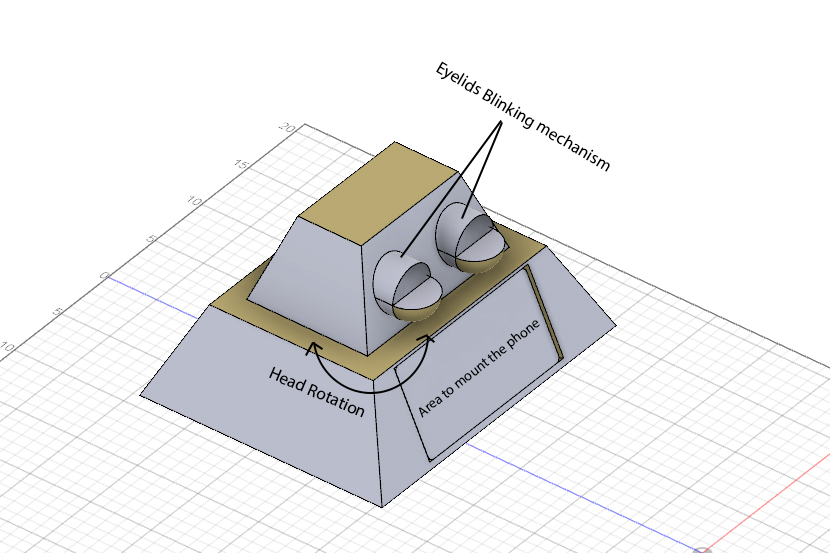
\includegraphics[scale=.5]{robot_image.jpg}
		\end{center}
	\end{figure}
\end{frame}
\begin{frame}
	\frametitle{Data Flow}
	\begin{figure}
		\begin{center}
			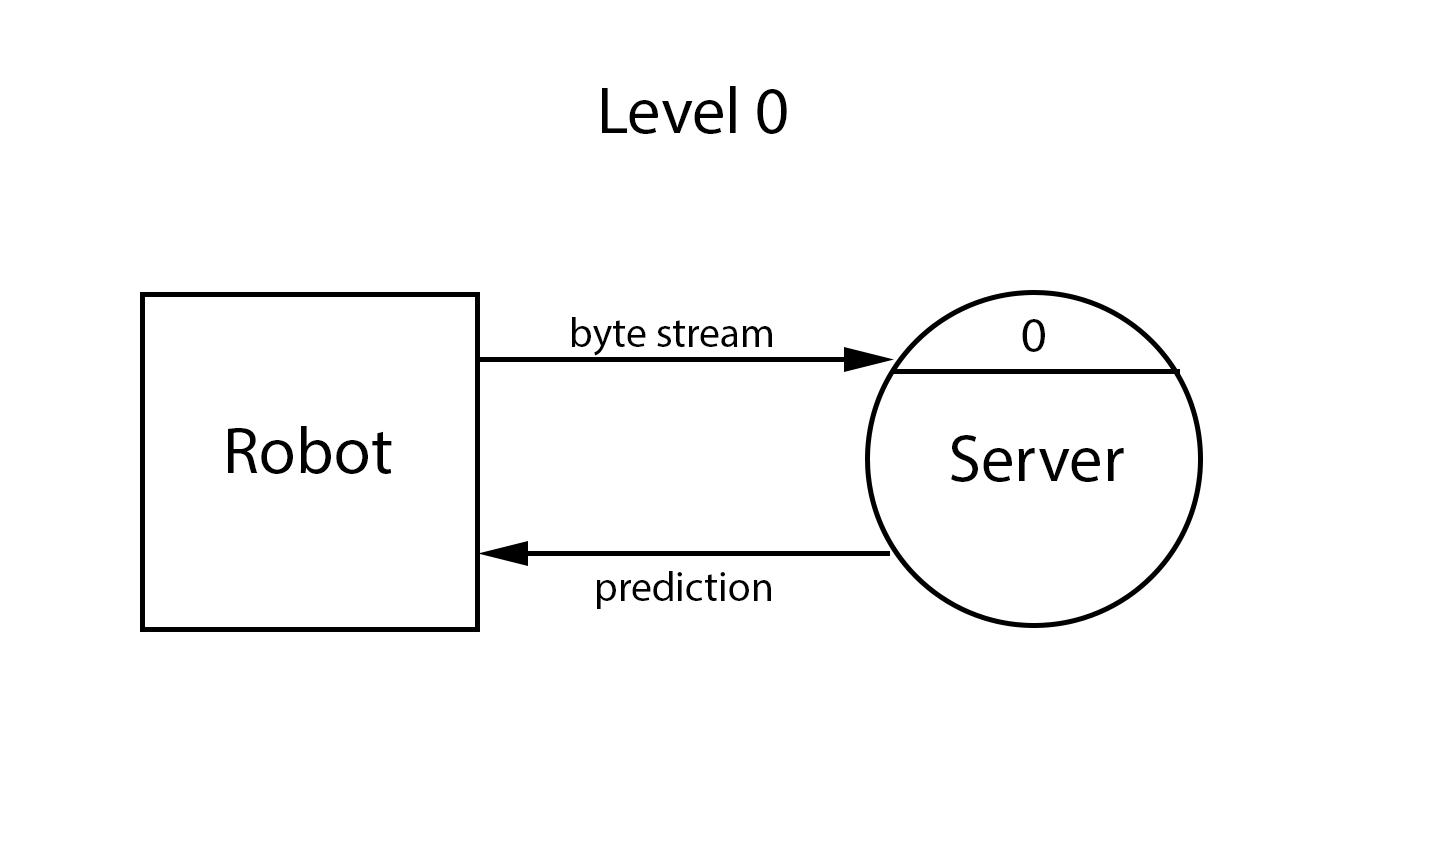
\includegraphics[scale=.7]{level_0_dia.jpg}
		\end{center}
	\end{figure}
\end{frame}
\begin{frame}
	\frametitle{Data Flow}
	\begin{figure}
		\begin{center}
			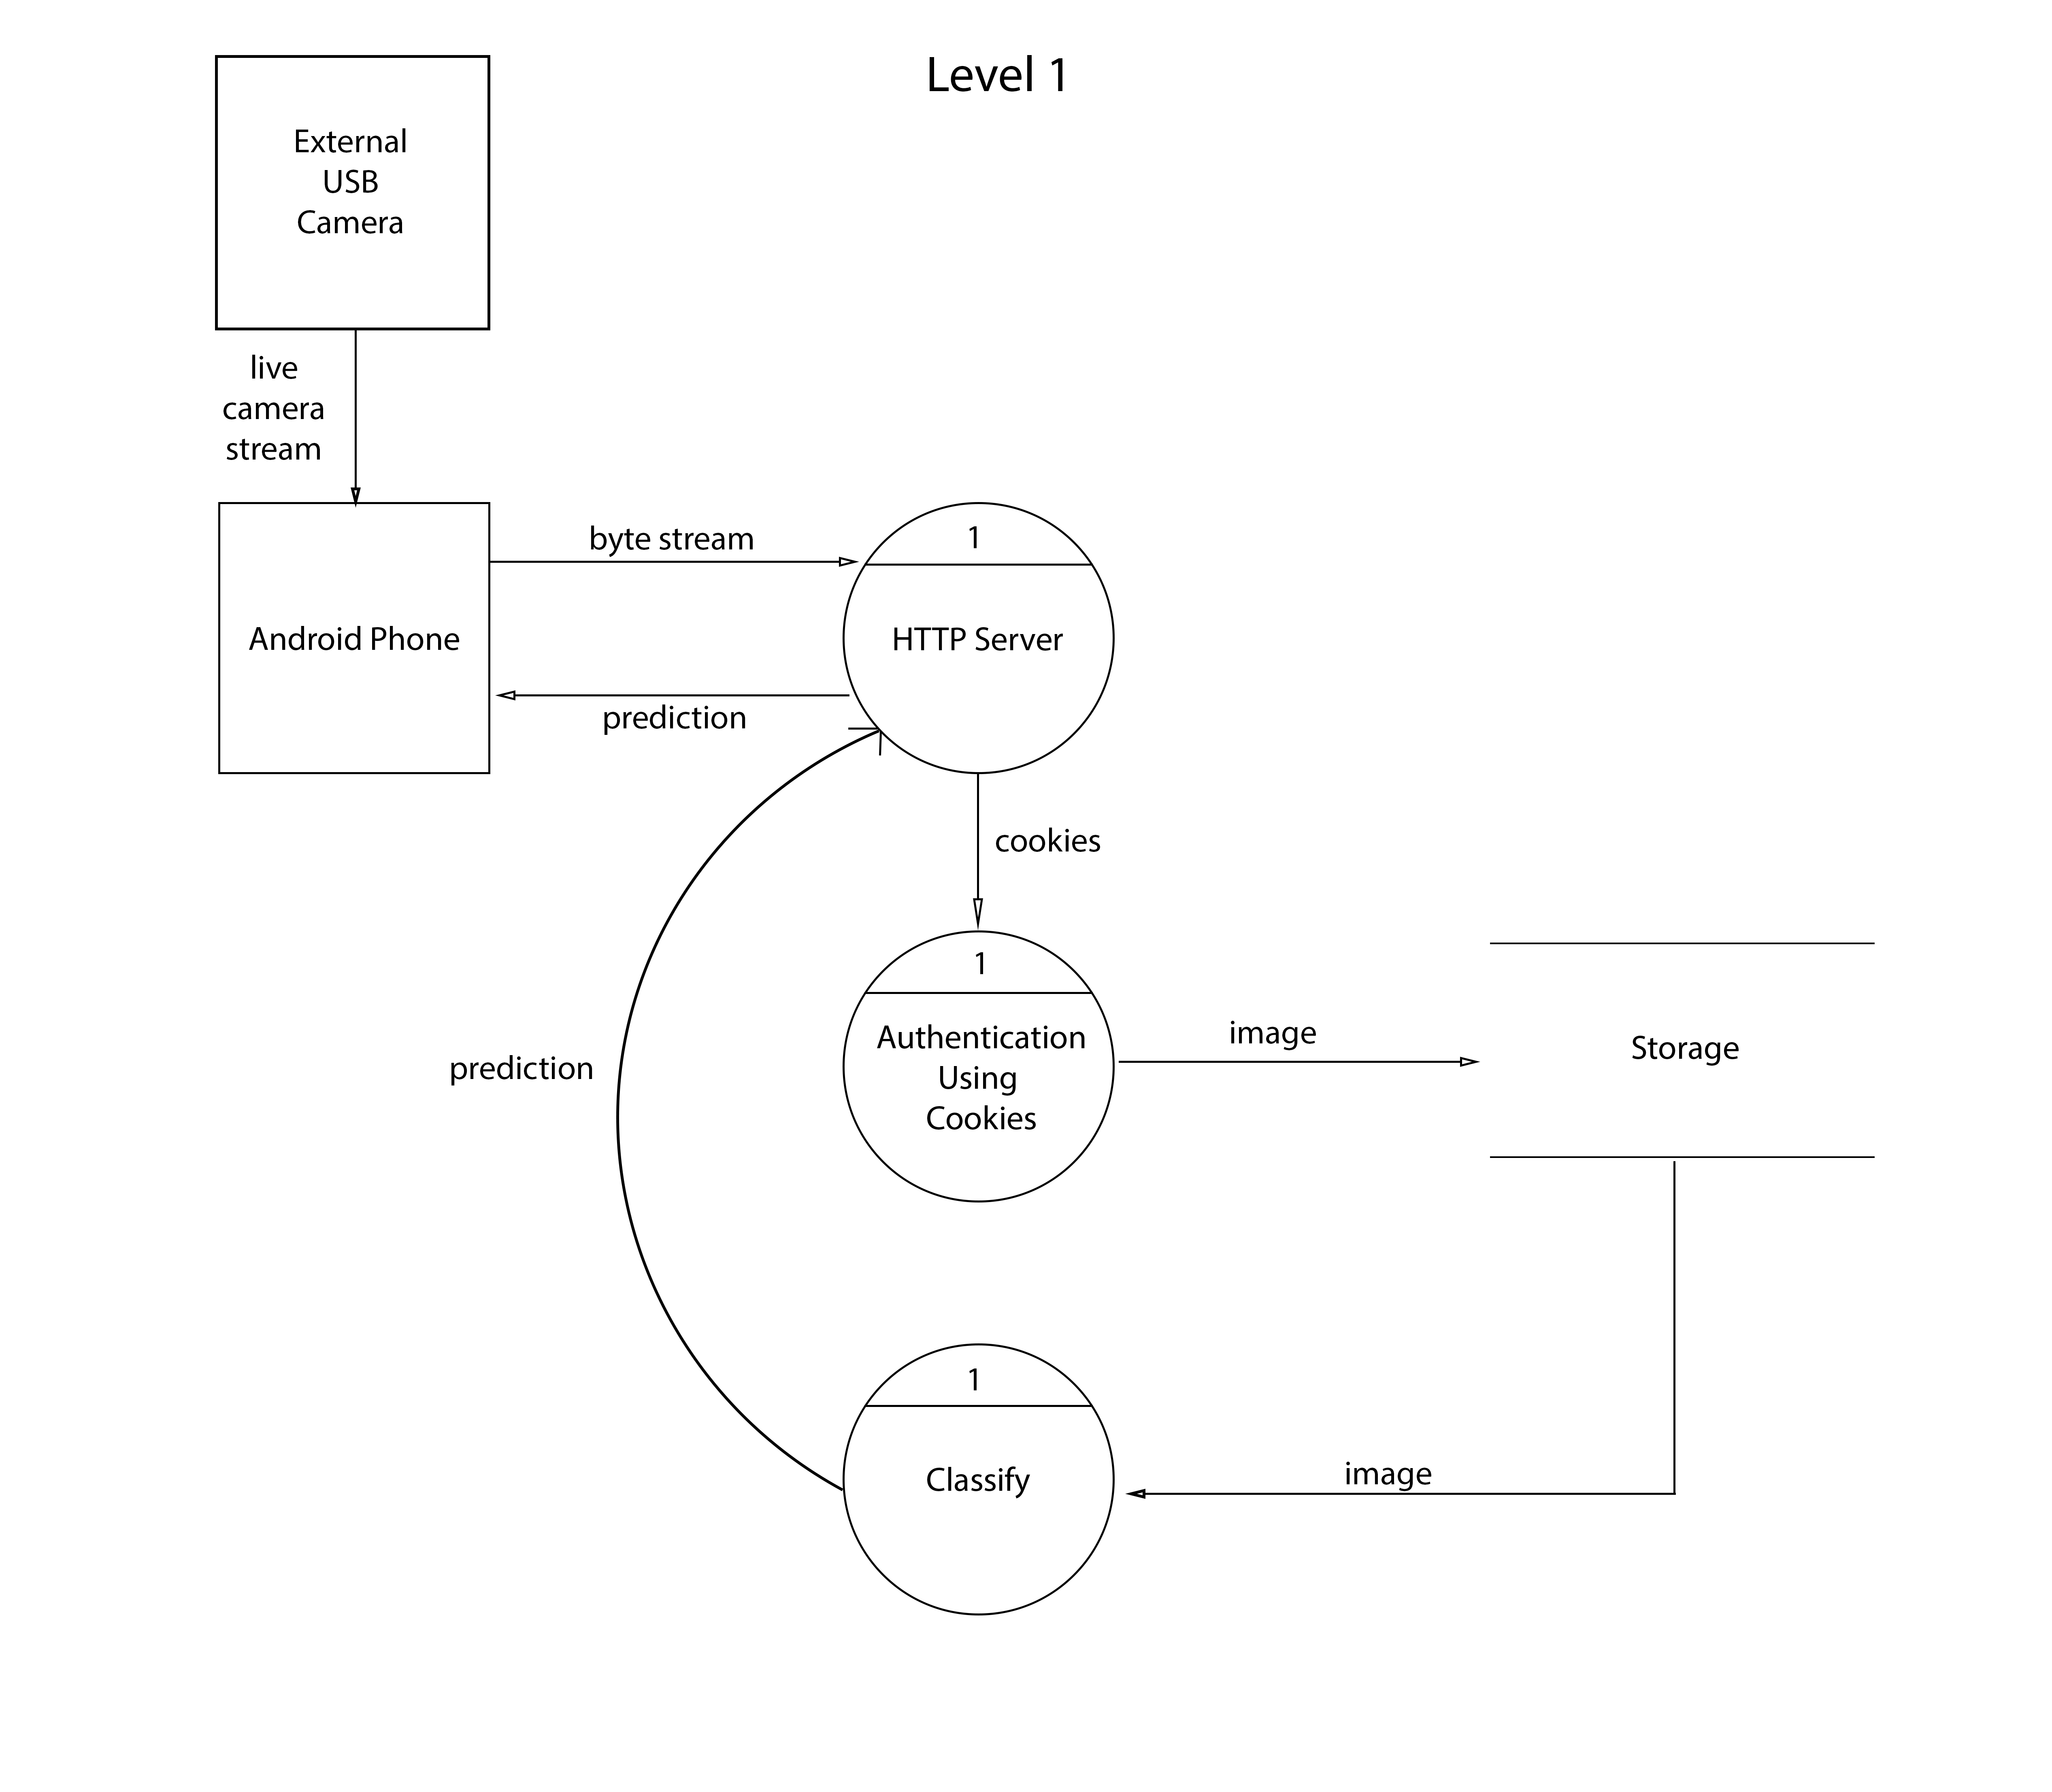
\includegraphics[scale=.21]{level_1_dia.jpg}
		\end{center}
	\end{figure}
\end{frame}

\begin{frame}
	\frametitle{UML Deployment Diagram}
	\begin{figure}
		\begin{center}
			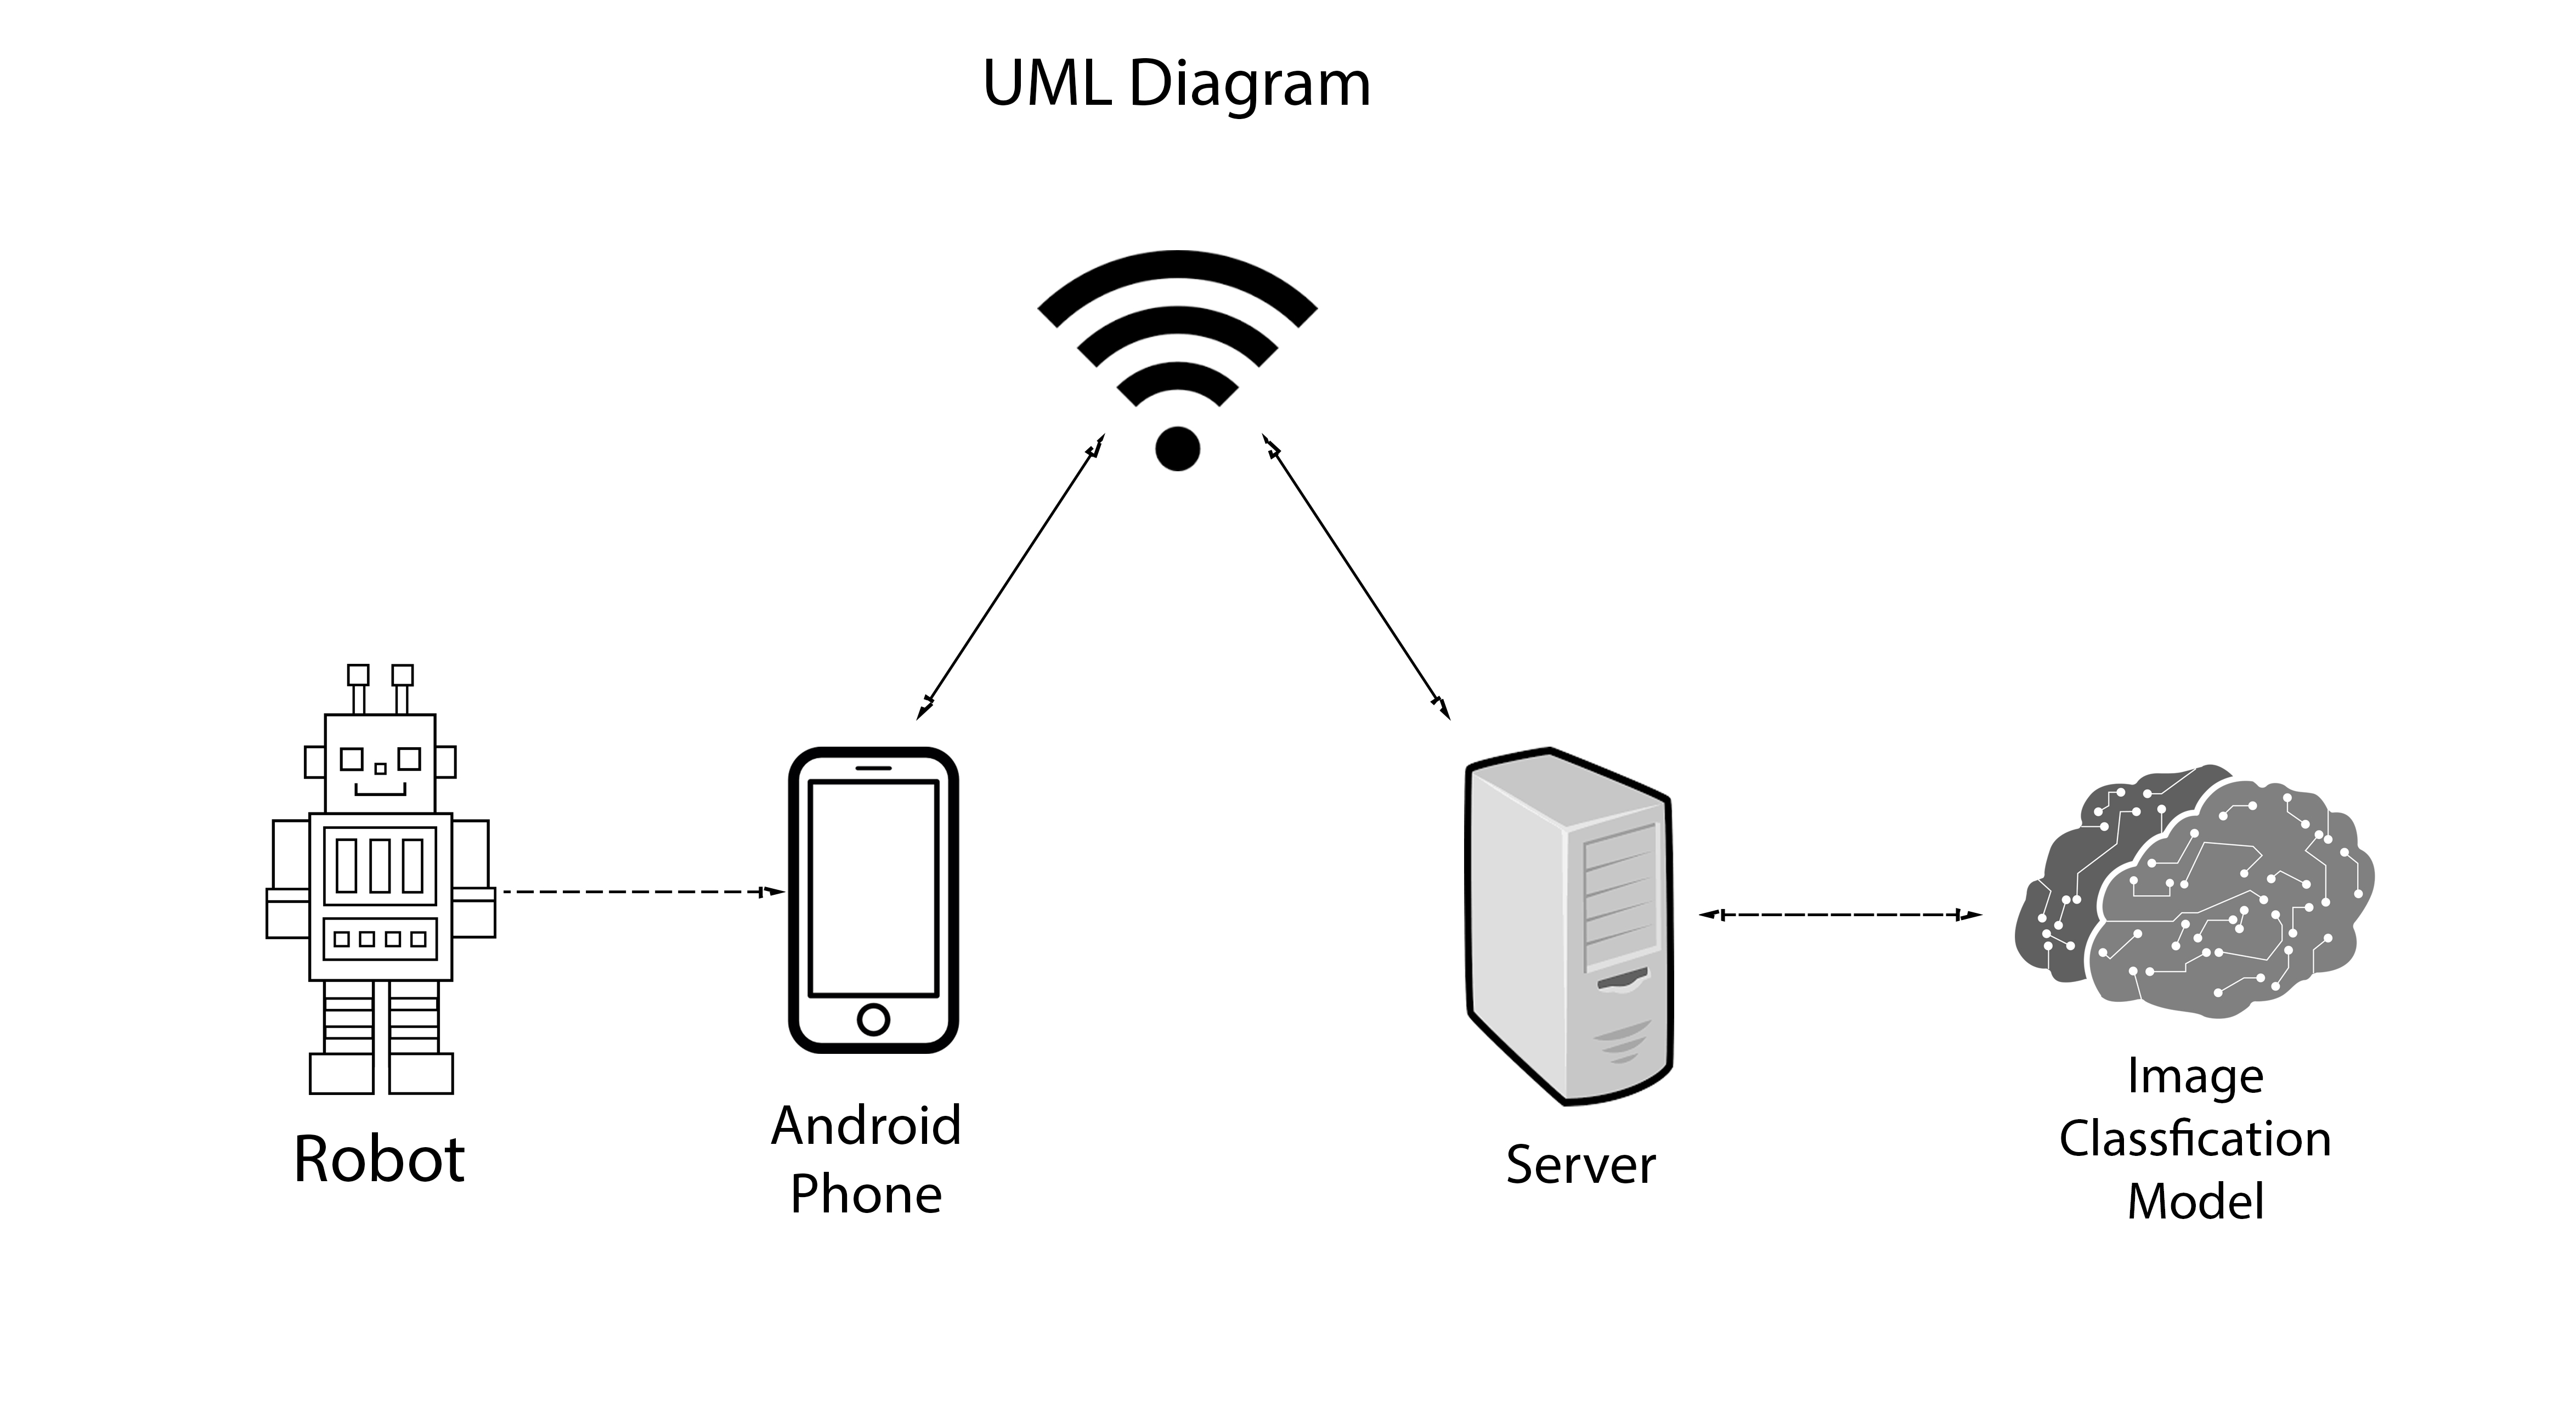
\includegraphics[scale=.3]{uml_dia.jpg}
		\end{center}
	\end{figure}
\end{frame}


\begin{frame}
	\frametitle{Use Case Diagram}
	\begin{figure}
		\begin{center}
			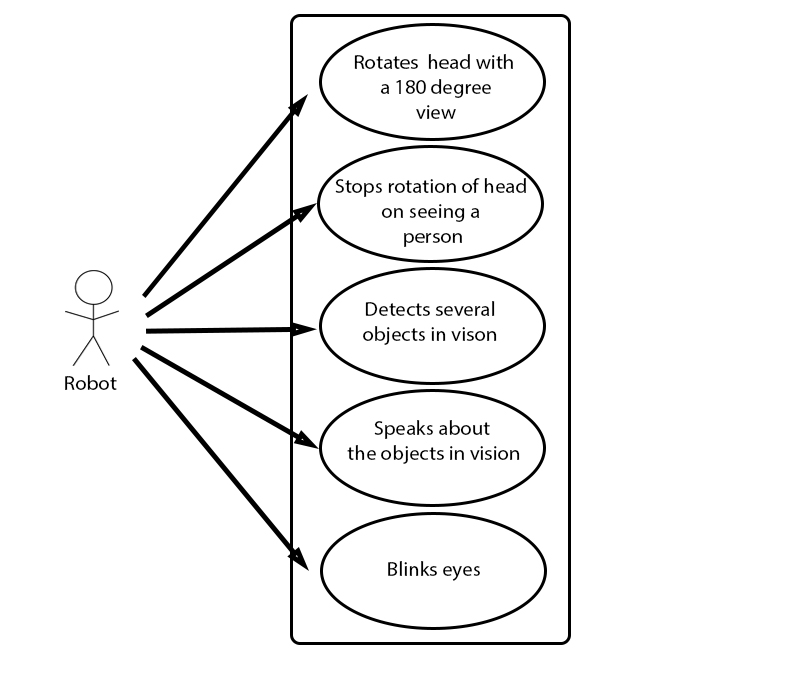
\includegraphics[scale=1.0]{usecase.jpg}
		\end{center}
	\end{figure}
\end{frame}

\section{Completed Tasks}
\begin{frame}{Task 1}
\begin{itemize}
  \item Create an android application and render the camera frames on top of the OpenGL surface.
\end{itemize}
\end{frame}

\begin{frame}{Task 2}
\begin{itemize}
  \item Classify Documents using SVM classifier from sklearn library.
  \item Predict the accuracy of classification.
\end{itemize}
\end{frame}


\begin{frame}{Task 3}
\begin{itemize}
  \item Create a server.
  \item Create an android app to capture images and send it to the server.
  \item Convert the image to grayscale and sent it back to the app.
\end{itemize}
\end{frame}

\begin{frame}{Task 4}
\begin{itemize}
  \item Image classification using SVM Classifier. 
\end{itemize}
\end{frame}

\begin{frame}{Task 5}
\begin{itemize}
  \item Classify images sent from the android app in the server.
  \item Retrieve classification from server and display in app.
\end{itemize}
\end{frame}

\begin{frame}{Task 6}
\begin{itemize}
	\item Send live feed from android app to the server
	\item Detect objects on the go in the server and send back the predictions
\end{itemize}
\end{frame}


\begin{frame}{Task 7}
\begin{itemize}
  \item Using Grid Search Tuning technique to evaluate the correct combinations of classifier parameters for improved accuracy in classification.
  \item Scaling in-order to make the feature range between 0 and 1.
  \item Replacing previous feature extraction methods with HOG.
\end{itemize}
\end{frame}


\begin{frame}{Task 8}
\begin{itemize}
	\item Fetch live stream from usb camera to the android app.
	\item The live classification on that data.
\end{itemize}
\end{frame}

\section{Results}
\begin{frame}
	\frametitle{Results}
	\begin{itemize}
		\item The outcome of the project is a social robot which can identify the objects seen in its vision.
		\item The robot, in its physical structure, has a 180 degree view made possible by its head movements.
		\item The robot performs a specific function of object classification.
		\item The live feed it retrieves from the usb camera attached to its eyes are fed to an android application on the phone.
		\item The app send the images to the server where it undergoes a number of processes as specified in the explanation of the project.
		\item Once the image classification is done, the robot speaks out what it sees.
	\end{itemize}
\end{frame}

\section{Conclusion}
\begin{frame}
	\frametitle{Conclusion}
	\begin{itemize}
		\item A social robot is an autonomous robot that interacts and communicates with humans or other autonomous physical agents by following social behaviors and rules attached to its role.
		\item This project successfully created a social robot, incorporated with human features such as, movement of head, closing of eyelids and speaking, and can identify and speak out about the objects seen through its vision, by making use of useful and popular computing domains such as Android, Machine learning, Image processing and Servers.
	\end{itemize}
\end{frame}
